\chapter{Opdracht 1: Projectopzet en analyse}

\section{Stap 1: Zet het project op}
Gebruik voor het project \textit{Java}, versie 11 of hoger.

Verder gebruiken we \textit{Maven}, een tool waarmee je Java-projecten kan opzetten
en gemakkelijk third-party dependencies, zoals frameworks en libraries, kunt 
gebruiken in je project. Zie hiervoor de pom.xml. Maven hoef je niet per se te 
installeren. We kunnen hiervoor onze Integrated Development Environment (IDE) gebruiken.
Ook is er een wrapper (mvnw) opgenomen in het project mocht je de commandline willen gebruiken (aanrader!). 

\subsection{Clone het project}
Clone het GitHub-project via de link die op Canvas wordt aangeboden.
We gebruik hiervoor private repositories binnen GitHub Education.
Zorg dat je een clone krijgt binnen GitHub om je werk in te leveren 
en op je machine om te werken. Open de root-directory van het project
via IntelliJ.

\subsection{Neem de opdrachtbeschrijving door}
Neem de opdrachtbeschrijving en de opdracht op Canvas door. 
Kan je (voor jezelf) antwoord geven op de volgende vragen?

\begin{enumerate}
    \item Wat moeten we precies maken?
    \item Waarom is er gekozen voor een web-applicatie?
    \item Hoe werkt blackjack ongeveer?
    \item Wat ga je ongeveer leren met deze cursus?
    \item Waar word je op beoordeeld?
    \item Waar krijg je de meeste punten voor?
    \item Wat moet je doen voor een voldoende?
\end{enumerate}

In het verleden is gebleken dat veel studenten erg laat beginnen 
en daarmee in de knoop komen met andere cursussen. Probeer dat te 
voorkomen door regelmatig je werk in te leveren, zodat je continu feedback 
kunt krijgen. Het is dus handig om voor jezelf een planning te maken.
De opdracht is om die reden opgedeeld in 6 stappen die ongeveer gelijk lopen 
met de inhoudelijke invulling van de werkcolleges.
Maak je je op enig punt tijdens de cursus zorgen over de planning,
geef het aan!

\subsection{Extra informatie: de projectstructuur}
Studenten hebben aangegeven meer informatie te willen ontvangen over hoe het 
systeem is opgezet. Daar is dit onderdeel voor bedoeld. Het is niet 
erg als je nog niet alles helemaal begrijpt of dat je niet overtuigd 
bent van deze opzet. Het gaat erom dat je in hoofdlijnen doorhebt 
waar wat te vinden is. Tijdens deze cursus gaan we er dieper op in.

Laten we eens kijken naar hoe het project is opgezet.
Onder src/main/java zien we onze packagestructuur.
Met behulp van packages kunnen we ons systeem op een logische manier 
ordenen. Dit is een belangrijke stap in het bereiken van 
\textit{separation of concerns, high cohesion en loose coupling}!

Structurele kwaliteit ziet immers op de onderhoudbaarheid
van een softwareproject. Een softwareproject heeft in algemene zin 
een goede structuur als deze is opgedeeld in kleine,
opzichzelf staande modules die intern veel samenhang 
en met elkaar beperkt koppeling vertonen.

\subsubsection{Packagestructuur in Java}
In Java kunnen we modules groeperen door gebruik te maken van 
\emph{packages} (in C\# en andere talen met \emph{namespaces}).
De naam van een Java-package lijkt op een soort omgekeerd webadres
en komt overeen met de onderliggende mappenstructuur.
Het is gebruikelijk om in Java-packages eerst te beginnen met de organisatienaam,
bijvoorbeeld \texttt{nl.hu.bep2}, en vervolgens de projectnaam \texttt{casino}.
Dan kunnen we het project opdelen in componenten, zoals in het casino-project: 
\begin{itemize}
\item \texttt{nl.hu.bep2.casino.chips}
\item \texttt{nl.hu.bep2.casino.blackjack}
\item \texttt{nl.hu.bep2.casino.security} (later)
\end{itemize}

Binnen elk component kan met packages 
onderscheid gemaakt worden naar het soort logica volgens een gelaagde aanpak. 
Dat leidt bij het casino-project tot de volgende 
mappen- en packagestructuur onder \texttt{src/main/java}:

\dirtree{%
    .1 nl.hu.bep2.casino.
        .2 chips.
            .3 application.
            .3 domain.
                .4 exception.
        .2 blackjack.
            .3 (...).
}

Het project is dus eerst opgedeeld in verschillende componenten en vervolgens in 
lagen. Voor nu is de splitsing in lagen gebaseerd op een 'application'-laag waarin 
we expliciet de verschillende usecases een plekje geven, en een 'domein'-laag waar 
we een domeinmodel realiseren (de ingrediënten van de usecases, zeg maar).

\subsection{Voorbeeld: Use cases van het chips-component}
Het chips-component biedt al een aantal use cases aan binnen ons systeem.
Deze zijn opgesomd in de ChipsService en laten zich gemakkelijk in een 
use case diagram vatten, zie: Figuur~\ref{fig:chips-use-cases}.
Kijk in de code of je dit kunt herkennen!

\begin{figure}[H]
    \centering
    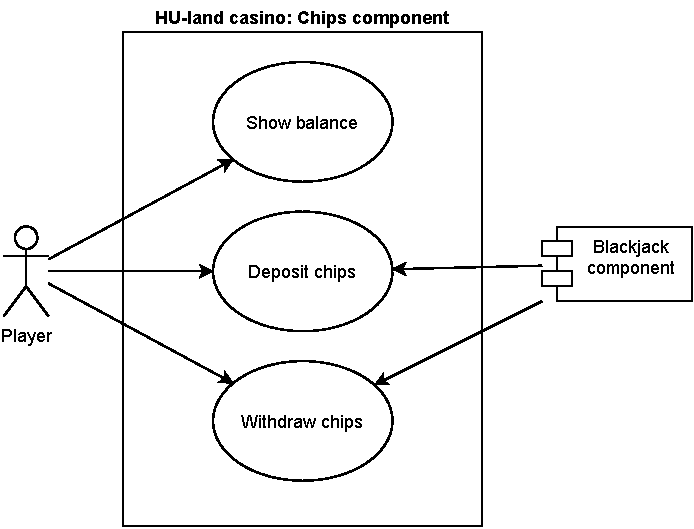
\includegraphics[height=0.4\linewidth]{chips-use-cases}
    \caption{De use cases van het chips-component}
    \label{fig:chips-use-cases}
\end{figure}

Zoals je ziet, willen we onze blackjack-component straks 
ook gebruik laten maken van de de chips-component!

\section{Stap 1: Analyseer de use cases van blackjack}
We hebben de opdracht doorgenomen en weten wat de opdrachtgever van ons verwacht.

We moeten ons voorstellen hoe blackjack precies werkt in de echte wereld.
Daarvan willen we een model maken in diagrammen en code, maar ook in ons hoofd!

Laten we een use case diagram maken, zodat de acties die door het systeem
aangeboden moeten worden voldoende duidelijk zijn. Hiervoor kan je het use case 
diagram van Figuur~\ref{fig:chips-use-cases} als inspiratie nemen.

\begin{figure}[H]
    \centering
    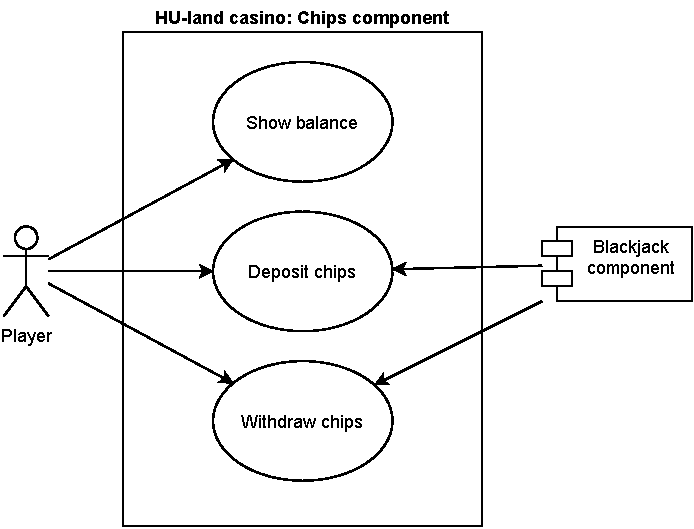
\includegraphics[height=0.4\linewidth]{chips-use-cases}
    \caption{De use cases van het chips-component}
    \label{fig:chips-use-cases}
\end{figure}

Neem de opdrachtbeschrijving door en denk na over de volgende zaken:
\begin{enumerate}
    \item Welke actors zijn er? Geautomatiseerde actors hoef je niet op te nemen.
    \item Wat wordt er binnen het component allemaal afgehandeld? Dit zijn geen use cases!
    \item Welke use cases moeten er naar buiten toe aangeboden worden om blackjack te kunnen spelen?
\end{enumerate}

Gebruik een tool als \textit{diagrams.net}, \textit{software ideas modeler} of \textit{visual paradigm},
sla het ontwerp op en exporteer het als \textit{.png} of \textit{.jpg}. 
Neem dit op in je projectdirectory (bijvoorbeeld onder een mapje \textit{diagrams}),
zodat je docent er naar kan kijken en er feedback op kan geven.

Commit je wijzigingen met een duidelijke naam, 
bijvoorbeeld: "Add use case diagram for blackjack". 
Push de wijzigingen naar je remote GitHub repository.

\section{Het objectmodel}
Wanneer je werkt met objecten, is het goed om het objectmodel van Booch in 
het achterhoofd te houden.\footnote{
    In de praktijk wordt ook wel eens verwezen naar de \textit{4 Pillars of Object Orientation}: 
    abstraction, encapsulation, polymorphism en inheritance. 
    Deze zijn in het objectmodel van Booch inbegrepen.
}

Het objectmodel van Booch onderscheidt vier belangrijke elementen 
die een rol spelen bij het object-georiënteerd modelleren:
\begin{enumerate}
    \item Abstraction
    \item Encapsulation 
    \item Modularity 
    \item Hierarchy
\end{enumerate}

Deze onderdelen noemen Booch et al. belangrijk omdat je 
zonder deze elementen geen object-georiënteerde taal (OO-taal) kan hebben.
Daarnaast beschrijven zij drie minder belangrijke elementen die je 
bij veel OO-talen tegen kunt komen: typing, persistence en concurrency.

Dit betekent natuurlijk niet dat je deze zaken buiten OO-talen niet tegen zal komen! 
Het objectmodel van Booch onderscheid een aantal zaken
die ons helpen goed gestructureerde object-georiënteerde software te ontwerpen.

Dit komt tijdens de colleges aan bod, maar kunnen we als volgt samenvatten:
\begin{enumerate}
    \item \textbf{Abstraction}: klassen en objecten zijn onze kernabstracties waarin we 
    toestand (fields) en gedrag (methods) samenbrengen die bij elkaar horen. Dit verhoogt \textit{cohesion}.
    We kunnen met deze abstracties communiceren via de publieke methoden. 
    De interne werking hoeven we dan niet te weten (\textit{implementation hiding}).
    \item \textbf{Encapsulation}: hoe een abstractie zijn toestand bijhoudt en zijn 
    gedrag uitvoert wordt afgeschermd van de buitenwereld. Om \textit{information hiding} te bereiken wordt 
    gebruik gemaakt van access modifiers (bijvoorbeeld: \textit{private}). 
    Dit beperkt \textit{coupling}. Wees spaarzaam met getters en setters (\textit{Tell, don't Ask}) 
    en wees niet afhankelijk van de onderdelen binnen een klasse \textit(\textit{Law of Demeter}).
    \item \textbf{Modularity}: klassen zijn modules waarin we toestand en gedrag samenbrengen. Daarnaast kennen 
    we interfaces om bepaald gedrag af te dwingen en enums om mogelijke waarden op te sommen. 
    Packages kunnen we gebruiken om klassen en andere modules te ordenen.
    \item \textbf{Hierarchy}: we kunnen packages onderbrengen in een logische, overzichtelijke ordening. Dat is onderdeel 
    van een softwarearchitectuur. Ook klassen en objecten kunnen in een hiërarchie tot elkaar staan. Er zijn namelijk 
    verschillende afhankelijkheden die tussen klassen kan gelden: \textit{dependency}, \textit{association}, \textit{aggregation},
    \textit{composition}, \textit{inheritance} en \textit{realisation}. Wat betreft inheritance en realisation zorgen 
    \textit{subtyping}, \textit{polymorphism} en \textit{dynamic binding} ervoor dat we een flexibele, uitwisselbare 
    invulling kunnen hebben van bepaalde abstracties. Eén abstractie kan namelijk verschillende vormen aannemen tijdens runtime:
    een subtype kan een implementatie of overschrijving verzorgen van het supertype.
\end{enumerate}

\section{Stap 2: Ontwerp een globaal domeinmodel}
Zodra je hebt nagedacht over de use cases en hier een model van hebt gemaakt,
kunnen we een overzicht maken van de concepten die we nodig hebben in ons blackjack-component.

Hiervoor kunnen we een versimpeld domeinmodel maken. 
Methods, attributes, rolnamen en multipliciteiten mag je achterwege laten.
Wees niet bang om veel concepten te modelleren!

Loop nogmaals door de opdrachtbeschrijving en verwerk de volgende zaken in je 
domeinmodel:
\begin{enumerate}
    \item Welke concepten leven er in de wereld van blackjack? 
    \item Wat zijn goede kandidaten voor klassen en enums?
    \item Wat zijn de relaties tussen deze concepten? Geef dit aan met de juiste pijlen.
    \item Welk concept kunnen we als centraal aanspreekpunt aanmerken waar we andere concepten aan kunnen hangen?
\end{enumerate}

Probeer hier niet teveel tijd aan te besteden.
Dit is een eerste opzet om het domein te structureren.
Tijdens het programmeren leren we meer over het domein, de functionaliteit en de structuur
en gaan we dit nader invullen en aanpassen!

Gebruik een tool als \textit{diagrams.net}, \textit{software ideas modeler} of \textit{visual paradigm},
sla het ontwerp op en exporteer het als \textit{.png} of \textit{.jpg}. 
Neem dit op in je projectdirectory (bijvoorbeeld onder een mapje \textit{diagrams}),
zodat je docent er naar kan kijken en er feedback op kan geven.

Commit je wijzigingen met een duidelijke naam, 
bijvoorbeeld: "Design initial domain model for blackjack". 
Push de wijzigingen naar je remote GitHub repository.

De docent geeft algemene of specifieke feedback
op basis waarvan je je domeinmodel kunt verbeteren.
Wat we alvast kunnen weggeven is dat je een spelpotje 
als centrale domeinklasse kan nemen.
